\documentclass[11pt, a4paper, jou]{apa7}
\setlength{\headheight}{14pt}
\usepackage[style=numeric, sorting=none]{biblatex}

\usepackage{hyperref}
\usepackage{url}
\usepackage{graphicx}
\usepackage{epstopdf}
\usepackage{amsmath}
\usepackage{float}

\usepackage{longtable}

\addbibresource{Ref.bib}

\leftheader{ZEHAO WANG}

\linespread{1.5}
\title{Will it rain tomorrow? --- Course Report on Weather Prediction}
\shorttitle{BIOS-7650 COURSE PROJECT}
\author{Zehao Wang}
\authorsaffiliations{Master student in Statistics, Department of Mathematics}
\course{BIOS-7650 Statistical Learning in Data Science}
\professor{Dr.\ Li. }
\duedate{\today}
\abstract{Whether it rains or not has the most direct impact on our daily life, therefore, the weather forecast is particularly important for us. The traditional approach to predict raining is to use computers combined with satellite cloud maps to solve a set of dynamical system equations\cite{teague2017evolution}. However, since the 21st century, the statistical learning approach has gradually become mainstream. Therefore, in this report, we try to use statistical learning methods (logistc regression, SVM and neural networks) to predict the weather. 
On the \href{https://www.kaggle.com/datasets/jsphyg/weather-dataset-rattle-package}{\emph{Rain in Australia}} dataset, we achieved an accuracy of about $85\%$ using these three statistical learning methods. This result is slightly higher than the current weather forecast accuracy (\href{https://www.forecastadvisor.com/Louisiana/NewOrleans/70112/}{forecasting accuracy in New Orleans}). And the code can be found in \href{https://github.com/Addasecond86/MS-Stat-Tulane/blob/main/Stat_Learning_in_Data_Analysis/Project/Code/Project_code.ipynb}{Github}. 
}
\begin{document}
\maketitle
\section{Methods}
The dataset we use is the \href{https://www.kaggle.com/datasets/jsphyg/weather-dataset-rattle-package}{\emph{Rain in Australia}} on Kaggle. It contains different weather indicators (e.g. temperature, humidity, wind direction, etc.) and whether it rained the next day for various regions of Australia for almost a decade, from October 2007 to June 2017. Before we make a prediction, the first thing we need to do is to clean the data. First, I dropped the subjects that had missing values in the variables \emph{RainToday} and \emph{RainTomorrow}. And I also dropped the subjects that contains missing value in categorical variables. For other continuous variables, it is not appropriate to fill the missing values with $0$, because variables such as temperature and barometric pressure cannot be $0$ even if they are missing. So I use the median of the current month to substitute the missing values of these continuous variables. 
\subsection{Logistic Regression}
    Logistic regression\cite{Berkson1944} is widely used in binary classification problems. Assume $p$ is the probability of rain tomorrow, then, for logistic regression, we have
    \begin{equation}
        \frac{p}{1-p}=\exp\left(\beta_0+\sum_{i=1}^{n}\beta_i x_i\right). 
    \end{equation}
    And we can estimate the coefficients $\beta_i$ by maximum likelihood estimation. 

    We first use all the variables except the date and interactions as predictor variables to predict whether it will rain tomorrow. Further, we use stepwise to explore whether the model can be further optimized. Akaike information criterion (AIC)\cite{Akaike1974} was used to see if any of the variables can be eliminated. AIC is a measure of the relative quality of statistical models for a given set of data. It is defined as following: 
    \begin{equation}
        \label{eq:AIC}
        {AIC} \,=\,2k-2\ln({\hat {L}}). 
    \end{equation}
    And $k$ is the number of estimated parameters in the model, $\hat{L}$ is the maximized value of the likelihood function for the model. So, the preferred model is the one with the minimum AIC value. 

    We also used Principal Component Analysis (PCA)\cite{Pearson1901} to extract features from the data. PCA is a method of reducing the dimensionality of data by transformation, which assumes that variables with higher variance carry more information. By reducing the dimensionality, we expect a significant increase in the classification accuracy. And because the absolute values of the variables are too different from each other, we should first transform the variables by (\ref{eq:trans}) to map them all to $[0,1]$. 
    \begin{equation}
        \label{eq:trans}
        X_{new} = \frac{X - X_{\min}}{X_{\max}- X_{\min}}. 
    \end{equation}
\subsection{SVM}
    Support Vector Machine (SVM) is a better method than logistic regression, it tries to maximize the margin between two different classes of data points. So it will have much lower risk on the test set. The optimization objectives of SVM are as following:  
    \begin{equation}
        \min_{|w|}\ y_{i}(\mathbf {w} ^{\mathsf {T}}\mathbf {x} _{i}-b)\geq 1,\ i=1, \cdots, n
    \end{equation}
    When the data is not linearly separable, we can add soft margins to it. The optimization goal then becomes the following: 
    \begin{equation}
        \min_{|w|}\ \lambda |\mathbf {w}| ^{2}+{\frac {1}{n}}\sum _{i=1}^{n}\max \left(0,1-y_{i}(\mathbf {w} ^{\mathsf {T}}\mathbf {x} _{i}-b)\right). 
    \end{equation}
    After that, we can transform it into a dual problem and then estimate the parameters by gradient descent. 

    For nonlinear data sets, we can use the kernel trick to map the original data to the projection space. And in projection space, we can separate them using a linear hyperplane. By using different kernel functions, we can project them into different spaces. The common kernel functions are polynomial kernel functions and Gaussian kernel functions. 

\subsection{Neural Network}
    In the 21st century, network-based approaches are undoubtedly the mainstream of machine learning. Considering the complexity of the data, we only use a simple fully connected network with two hidden layers. Its structure is shown in Figure~(\ref{fig:NN}). In this network, the activation functions of both fully connected hidden layers are ReLU\cite{Lu2020} (\ref{eq:ReLU}). It can solve the gradient disappearance or explosion problem in some extent. 
    \begin{equation}
        \label{eq:ReLU}
        ReLU(x) = \max(0,x)
    \end{equation}
    Also, Sigmoid is used as the activation function (\ref{eq:sigmoid}) in the output layer. Therefore, the final output we get is an output in $(0,1)$, and we consider values greater than $0.5$ as $1$, otherwise as $0$. 
    \begin{equation}
        \label{eq:sigmoid}
        Sigmoid(x) = \frac{1}{1+e^{-x}}
    \end{equation}
    The optimization algorithm for neural network parameters is Backpropagation\cite{goodfellow20166}. It uses the chain derivative rule to complete the update of the parameters. Since we are dealing with a binary classification problem, we use binary cross-entropy (\ref{eq:binary cross_entropy}) as the loss function. 
    \begin{equation}
        \label{eq:binary cross_entropy}
        L = -\frac{1}{n}\sum_{i=1}^{n}(y_i\ln(p_i)+(1-y_i)\ln(1-p_i))
    \end{equation}
    It can be seen that the more $p(y)$ matches with $y$, the closer the loss function is to $0$. On the contrary, it is infinite. 

\section{Results}

\subsection{Logistic Regression}
    Using $60\%$ as training set and $40\%$ as test set, logistic regression model with all the variables except the date has an accuracy of $85.365\%$ on the test set. And the accuracy on train set is $85.325\%$. The Confusion matrix is shown in Figure~(\ref{fig:logistic_confusion}). The accuracy and recall of this model are shown in Table~(\ref{tab:logistic_summary}). It can be seen that the accuracy ($0.88$) and recall ($0.95$) of the model are quite high with \emph{RainTomorrow} as \emph{No}. But it doesn't do well on data with \emph{RainTomorrow} as \emph{Yes}. 

    Next, we start from the full model and use AIC as a criterion to see if any variables can be excluded. The full process of stepwise is shown in Table~(\ref{tab:model_selection_aic}). Unfortunately, the AIC value of the full model is the smallest, so we cannot exclude any variables. 

\subsection{SVM}
We used the same training and testing data on this method. Using SVM without kernel trick, the accuracy obtained on the test set is $85.272\%$. And the training accuracy is $85.170\%$. This result is basically the same as the logistic regression. It also shows that some of the data in our dataset are linearly inseparable. Its confusion matrix is shown in Figure~(\ref{fig:SVM_confusion}), and the accuracy and recall are shown in Table~(\ref{tab:SVM_summary}); It can also be seen that SVM has no improvement over logistic regression. 

The reason for no improvement in classification accuracy may be that the data itself is linearly inseparable. So we try to introduce two kernel functions (polynomial and Gaussian). The results are shown in Figure~(\ref{fig:SVM_poly_confusion}), (\ref{fig:SVM_gauss_confusion}) and Table~(\ref{tab:SVM_poly_summary}), (\ref{tab:SVM_gauss_summary}). However, based on the classification results, the accuracy of both methods on the test set is slightly lower. This is probably because the two kernel functions cannot separate these two classes of data. 

However, in general, SVM should perform better, so we tried to use PCA to extract features first, and then use the model to classify the data. Using PCA, we chose to retain $85\%$ of the information, and we reduced the original 114-dimensional data to 64 dimensions. The classification results on this data are shown in Table~(\ref{tab:Logit_PCA_summary}), (\ref{tab:SVM_PCA_summary}), (\ref{tab:SVM_poly_PCA_summary}), (\ref{tab:SVM_gauss_PCA_summary}). 
Unfortunately, however, these results indicate that the accuracy on the test set does not increase, but decreases slightly. At the same time, SVM models with kernel trick show a further increase in training accuracy (SVM polynomial, train accuracy: $87.048\%$, test accuracy: $84.377\%$; SVM gaussian: train accuracy: $86.711\%$, test accuracy: $84.789\%$), but a decrease in test accuracy, indicating that overfitting has occurred. This means that PCA cannot lead to further improvement of accuracy. 



\subsection{Neural Network}
We used the same training and testing data and mapped the data to $(0,1)$ and started training. First, the network was trained with $50$ Epochs. The loss of the model on the test set and the loss on the validation set during the training process are shown in Figure~(\ref{fig:NN_process_50}). It can be seen that, although the training loss keeps decreasing, the loss on the validation set stops decreasing after $20$ Epochs. Then, we can see that it even starts to increase after $30$ Epochs. This indicates that the overfitting starts after $20$ Epochs. So, we retrain a $20$ Epochs network. And the training process is shown as Figure~(\ref{fig:NN_process_20}). It can be seen from the figure that overfitting has not occurred. The performance of this network on the test set is shown in Figure~(\ref{fig:FC_confusion_matrix}) and Table~(\ref{tab:FC_summary}). In the end, we obtained an accuracy of $85.9995\%$ on the test set. This accuracy is a little higher than either logistic regression or SVM. 

\section{Discussion}

As you can see, we use three different approaches. But the results are basically the same, that is, we can only achieve an accuracy of less than $86\%$ at most. This seems very frustrating, because the error rate is about $15\%$. This means that on average the prediction will be wrong one day out of a week. 

However, this is about the level of accuracy of current weather predictions. You can see the accuracy of the weather predictions for New Orleans last year on this \href{https://www.forecastadvisor.com/Louisiana/NewOrleans/70112/}{website}. As shown in Figure~(\ref{fig:weather_prediction_nola}), this website shows that the highest channel for 2021 weather prediction accuracy in the New Orleans area is just $84.92\%$. 

In addition, we can see that the accuracy and recall of the three models are higher for not raining weather than raining weather. This means that when the weather prediction says it will not rain, then it is very likely that it will not rain. But when the prediction says it will rain, then there is also a chance that it will not rain. Therefore, to avoid the second error case, which occurs more frequently, the weather forecast is now given in the form of rainfall probabilities. 

On the other hand, due to the interpretability of the logistic regression model, we can see which variable causes the most significant change in the probability of raining after mapping each variable to $[0,1]$. The first 13 coefficients with the largest absolute values are shown in Table~(\ref{tab:rank_coef}). From the table, we can see that the pressure at 3pm is negatively correlated with raining, while the wind speed and the humidity at 3pm are positively correlated. 

Finally, for further improvement, the date variable could be added to turn our data into a time series. On this basis, it might be useful to consider adding periodic factors such as seasonality to the forecasting model. Also, interactions can be introduced in the logistic regression model. 

\printbibliography 
\clearpage
\appendix
\section{Figures and Tables}
\begin{figure}[h]
    \centering
    \caption{Confusion matrix of logistic regression model. $0$ means not raining and $1$ means raining. And darker colors indicate larger numbers. }\label{fig:logistic_confusion}
    \includegraphics[width=.45\textwidth]{figures/Logit_confusion_matrix.eps}
\end{figure}

\begin{figure}[h]
    \centering
    \caption{Confusion matrix of SVM. }\label{fig:SVM_confusion}
    \includegraphics[width=.45\textwidth]{figures/SVM_confusion_matrix.eps}
\end{figure}

\begin{figure}[h]
    \centering
    \caption{Confusion matrix of SVM with polynomial kernel function. }\label{fig:SVM_poly_confusion}
    \includegraphics[width=.45\textwidth]{figures/SVM_poly_confusion_matrix.eps}
\end{figure}

\begin{figure}[h]
    \centering
    \caption{Confusion matrix of SVM with gaussian kernel function. }\label{fig:SVM_gauss_confusion}
    \includegraphics[width=.45\textwidth]{figures/SVM_gauss_confusion_matrix.eps}
\end{figure}

\begin{table}[h]
    \centering
    \caption{Classification results of logistic regression models on the test set. }
    \label{tab:logistic_summary}
    \resizebox{\columnwidth}{!}{%
    \begin{tabular}{rrrrr}
    \hline
                 & precision & recall & f1-score & support \\ \hline
    Not Raining  & 0.87      & 0.95   & 0.91     & 38571   \\
    Raining      & 0.73      & 0.53   & 0.62     & 10913    \\
    accuracy     &           &        & 0.85     & 49484   \\
    macro avg    & 0.80      & 0.74   & 0.76     & 49484   \\
    weighted avg & 0.84      & 0.85   & 0.84     & 49484   \\ \hline
    \end{tabular}%
    }
\end{table}

\begin{table}[h]
    \centering
    \caption{Classification results of SVM on the test set. }
    \label{tab:SVM_summary}
    \resizebox{\columnwidth}{!}{%
    \begin{tabular}{rrrrr}
    \hline
                 & precision & recall & f1-score & support \\ \hline
    Not Raining  & 0.87      & 0.95   & 0.91     & 38571   \\
    Raining      & 0.74      & 0.51   & 0.61     & 10913    \\
    accuracy     &           &        & 0.85     & 49484   \\
    macro avg    & 0.81      & 0.73   & 0.76     & 49484   \\
    weighted avg & 0.84      & 0.85   & 0.84     & 49484   \\ \hline
    \end{tabular}%
    }
\end{table}

\begin{table}[h]
    \centering
    \caption{Classification results of SVM with polynomial kernel function on the test set. }
    \label{tab:SVM_poly_summary}
    \resizebox{\columnwidth}{!}{%
    \begin{tabular}{rrrrr}
    \hline
                 & precision & recall & f1-score & support \\ \hline
    Not Raining  & 0.85      & 0.96   & 0.91     & 38571   \\
    Raining      & 0.76      & 0.41   & 0.61     & 10913    \\
    accuracy     &           &        & 0.84     & 49484   \\
    macro avg    & 0.81      & 0.69   & 0.72     & 49484   \\
    weighted avg & 0.83      & 0.84   & 0.82     & 49484   \\ \hline
    \end{tabular}%
    }
\end{table}

\begin{table}[h]
    \centering
    \caption{Classification results of SVM with gaussian kernel function on the test set. }
    \label{tab:SVM_gauss_summary}
    \resizebox{\columnwidth}{!}{%
    \begin{tabular}{rrrrr}
    \hline
                 & precision & recall & f1-score & support \\ \hline
    Not Raining  & 0.85      & 0.97   & 0.90     & 38571   \\
    Raining      & 0.79      & 0.37   & 0.51     & 10913    \\
    accuracy     &           &        & 0.84     & 49484   \\
    macro avg    & 0.82      & 0.67   & 0.71     & 49484   \\
    weighted avg & 0.83      & 0.84   & 0.82     & 49484   \\ \hline
    \end{tabular}%
    }
\end{table}
    
\begin{table}[h]
    \centering
    \caption{Model selection for logistic regression with AIC as criterion. Full model has the smallest AIC. }
    \label{tab:model_selection_aic}
    \begin{tabular}{lrrr}
    \hline
                   & Df & Deviance & AIC                          \\ \hline
    Full Model     &    & 84120    & {\color[HTML]{FE0000} 84338} \\
    -Temp3pm       & 1  & 84130    & 84346                        \\
    -Cloud9am      & 1  & 84131    & 84347                        \\
    -Evaporation   & 1  & 84131    & 84347                        \\
    -Humidity9am   & 1  & 84135    & 84351                        \\
    -WindGustDir   & 15 & 84168    & 84356                        \\
    -MinTemp       & 1  & 84148    & 84364                        \\
    -Temp9am       & 1  & 84152    & 84368                        \\
    -WindSpeed9am  & 1  & 84174    & 84390                        \\
    -Rainfall      & 1  & 84175    & 84391                        \\
    -MaxTemp       & 1  & 84219    & 84435                        \\
    -WindDir9am    & 15 & 84311    & 84499                        \\
    -WindDir3pm    & 15 & 84324    & 84512                        \\
    -WindSpeed3pm  & 1  & 84471    & 84687                        \\
    -RainToday     & 1  & 84491    & 84707                        \\
    -Sunshine      & 1  & 84538    & 84754                        \\
    -Cloud3pm      & 1  & 84799    & 85015                        \\
    -Pressure9am   & 1  & 84819    & 85035                        \\
    -Pressure3pm   & 1  & 85390    & 85606                        \\
    -Location      & 46 & 86542    & 86668                        \\
    -WindGustSpeed & 1  & 87585    & 87801                        \\
    -Humidity3pm   & 1  & 87949    & 88165                        \\ \hline
    \end{tabular}
\end{table}

\begin{table}[h]
    \centering
    \caption{Classification results of logistic regression model using PCA on the test set. }
    \label{tab:Logit_PCA_summary}
    \resizebox{\columnwidth}{!}{%
    \begin{tabular}{rrrrr}
    \hline
                 & precision & recall & f1-score & support \\ \hline
    Not Raining  & 0.86      & 0.94   & 0.90     & 38571   \\
    Raining      & 0.69      & 0.45   & 0.54     & 10913    \\
    accuracy     &           &        & 0.83     & 49484   \\
    macro avg    & 0.77      & 0.70   & 0.72     & 49484   \\
    weighted avg & 0.82      & 0.83   & 0.82     & 49484   \\ \hline
    \end{tabular}%
    }
\end{table}

\begin{table}[h]
    \centering
    \caption{Classification results of SVM using PCA on the test set. }
    \label{tab:SVM_PCA_summary}
    \resizebox{\columnwidth}{!}{%
    \begin{tabular}{rrrrr}
    \hline
                 & precision & recall & f1-score & support \\ \hline
    Not Raining  & 0.85      & 0.95   & 0.90     & 38571   \\
    Raining      & 0.71      & 0.41   & 0.52     & 10913    \\
    accuracy     &           &        & 0.83     & 49484   \\
    macro avg    & 0.78      & 0.68   & 0.71     & 49484   \\
    weighted avg & 0.82      & 0.83   & 0.82     & 49484   \\ \hline
    \end{tabular}%
    }
\end{table}

\begin{table}[h]
    \centering
    \caption{Classification results of SVM with polynomial kernel function and using PCA on the test set. }
    \label{tab:SVM_poly_PCA_summary}
    \resizebox{\columnwidth}{!}{%
    \begin{tabular}{rrrrr}
    \hline
                 & precision & recall & f1-score & support \\ \hline
    Not Raining  & 0.86      & 0.96   & 0.91     & 38571   \\
    Raining      & 0.74      & 0.45   & 0.56     & 10913    \\
    accuracy     &           &        & 0.84     & 49484   \\
    macro avg    & 0.80      & 0.70   & 0.73     & 49484   \\
    weighted avg & 0.83      & 0.84   & 0.83     & 49484   \\ \hline
    \end{tabular}%
    }
\end{table}

\begin{table}[h]
    \centering
    \caption{Classification results of SVM with gaussian kernel function and using PCA on the test set. }
    \label{tab:SVM_gauss_PCA_summary}
    \resizebox{\columnwidth}{!}{%
    \begin{tabular}{rrrrr}
    \hline
                 & precision & recall & f1-score & support \\ \hline
    Not Raining  & 0.86      & 0.96   & 0.91     & 38571   \\
    Raining      & 0.75      & 0.47   & 0.57     & 10913    \\
    accuracy     &           &        & 0.83     & 49484   \\
    macro avg    & 0.81      & 0.71   & 0.74     & 49484   \\
    weighted avg & 0.84      & 0.85   & 0.83     & 49484   \\ \hline
    \end{tabular}%
    }
\end{table}

\begin{figure}[h]
    \centering
    \caption{Neural network structure. }\label{fig:NN}
    \includegraphics[width=.3\textwidth]{figures/Network_structure.png}
\end{figure}

\begin{figure}[h]
    \centering
    \caption{Training process with epoch $=50$. It can be seen that overfitting has occurred. }\label{fig:NN_process_50}
    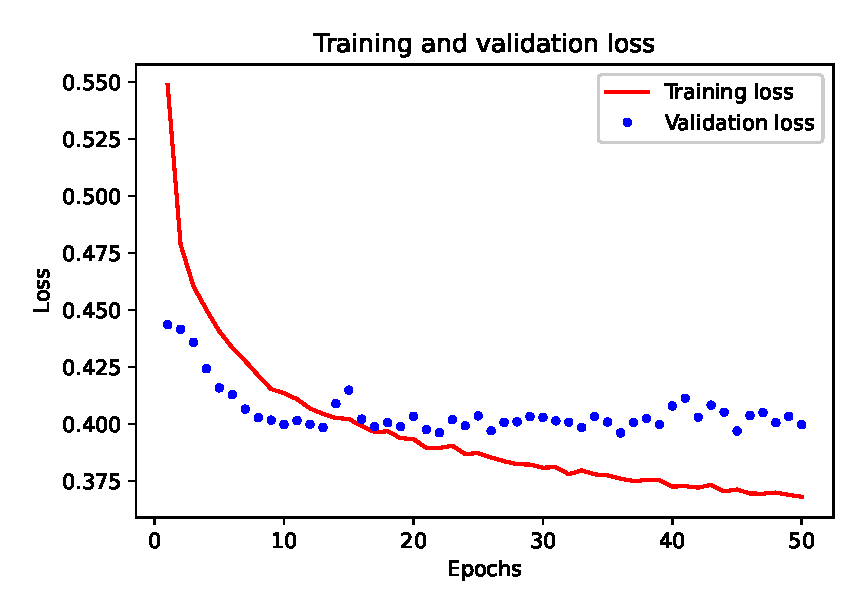
\includegraphics[width=.45\textwidth]{figures/error_50.eps}
\end{figure}

\begin{figure}[h]
    \centering
    \caption{Training process with epoch $=20$. }\label{fig:NN_process_20}
    \includegraphics[width=.45\textwidth]{figures/error_20.eps}
\end{figure}

\begin{figure}[h]
    \centering
    \caption{Confusion matrix of Neural Network. }\label{fig:FC_confusion_matrix}
    \includegraphics[width=.45\textwidth]{figures/FC_confusion_matrix.eps}
\end{figure}

\begin{table}[h]
    \centering
    \caption{Classification results of Neural Network on the test set. }
    \label{tab:FC_summary}
    \resizebox{\columnwidth}{!}{%
    \begin{tabular}{rrrrr}
    \hline
                 & precision & recall & f1-score & support \\ \hline
    Not Raining  & 0.89      & 0.93   & 0.91     & 38571   \\
    Raining      & 0.71      & 0.61   & 0.66     & 10913    \\
    accuracy     &           &        & 0.86     & 49484   \\
    macro avg    & 0.80      & 0.77   & 0.78     & 49484   \\
    weighted avg & 0.85      & 0.86   & 0.86     & 49484   \\ \hline
    \end{tabular}%
    }
\end{table}

\begin{figure}[h]
    \centering
    \caption{Weather prediction accuracy for New Orleans in 2021. The highest one has an accuracy of $84.92\%$. }\label{fig:weather_prediction_nola}
    \includegraphics[width=.55\textwidth]{figures/Weather2021.png}
\end{figure}

\begin{table}[h]
\centering
\caption{The first 13 variables with the largest absolute value of the coefficient. }
\label{tab:rank_coef}
\begin{tabular}{lrr}
\hline
Variables             & Coef   & AbsCoef \\ \hline
Pressure3pm           & -9.583 & 9.583   \\
WindGustSpeed         & 7.243  & 7.243   \\
Humidity3pm           & 6.232  & 6.232   \\
Pressure9am           & 5.913  & 5.913   \\
MaxTemp               & -2.384 & 2.384   \\
WindSpeed3pm          & -1.947 & 1.947   \\
Rainfall              & 1.899  & 1.899   \\
Temp3pm               & 1.523  & 1.523   \\
Sunshine              & -1.479 & 1.479   \\
Location\_MountGinini & -1.086 & 1.086   \\
Cloud3pm              & 1.074  & 1.074   \\
MinTemp               & 1.048  & 1.048   \\
Temp9am               & 1.022  & 1.022   \\ \hline
\end{tabular}
\end{table}

\end{document}